
We tested our optimization algorithms by modelling the behaviour of eleven resident killer whales off the coast of British Columbia, Canada using a HHMM. The data we use were collected in August and September of 2020 and consist of tri-axial acceleration over time. Observations were collected at a rate of 50 Hz using a CATS biologger (Customizable Animal Tracking Solutions, {\em{www.cats.is}}).

%Acceleration was measured in three dimensions, which together represent the complete range of movement of an animal (forward/backward, upward/downward, and right/left). Tri-axial acceleration readings are common in these types of tags and are often used to infer animal behaviour such as foraging \citep{Fehlmann:2017,Wright:2017,Cade:2017}. The act of attaching and detaching the tag caused anomalous behaviour before 1:20 p.m. and after 6:00 p.m., so observations taken during these time periods are ignored. There were also periods of time when the tag failed to record observations, resulting in data gaps between 2:25 p.m. and 2:37 p.m. and between 4:07 p.m. and 5:07 p.m. 

We divided the accelerometer data into two-second windows, each consisting of 100 accelerometer readings. We then performed a Fourier transform within each two-second window, and summarized the window with two measures of ``wiggliness":
(1) the sum of the squares of all Fourier coefficients corresponding to frequencies less than 5 Hz, and (2) the sum of the squares of all Fourier coefficients corresponding to frequencies greater than 5 Hz. The processed data set contains a total of $T=89462$ two-second windows.

We used an HHMM \citep{Barajas:2017} to model the killer whale biologging data for two reasons. First, fine-scale biologging data often exhibits multi-scale behaviour which can be accounted for by an HHMM \citep{Sidrow:2021}. Second, we wish to use our optimization algorithm on a more complicated model in addition to the simple Gaussian HMM from the case study. We selected a total of $N^{(c)} = 3$ coarse-scale states and $N^{(f,i)} = N^{(f)} = 3$ fine-scale states for each coarse-scale state. We enforce that the state-dependent fine-scale distributions are shared across coarse-scale states. In practice, the number of hidden states in a HMM should be selected using model selection and validation techniques as well as with the help of subject-matter experts \citep{Pohle:2017}. However, we are primarily interested in the performance of our optimization routines, so we select the number of hidden states to be in line with common values in the statistical ecology literature. 

Figure (\ref{fig:data}) shows the depth and wiggliness data corresponding to one of the whales. Depth and wiggliness are colour-coded by the most likely coarse- and fine-scale hidden states of each two-second window conditioned on the MLE parameters.
%
\begin{figure}
    \centering
    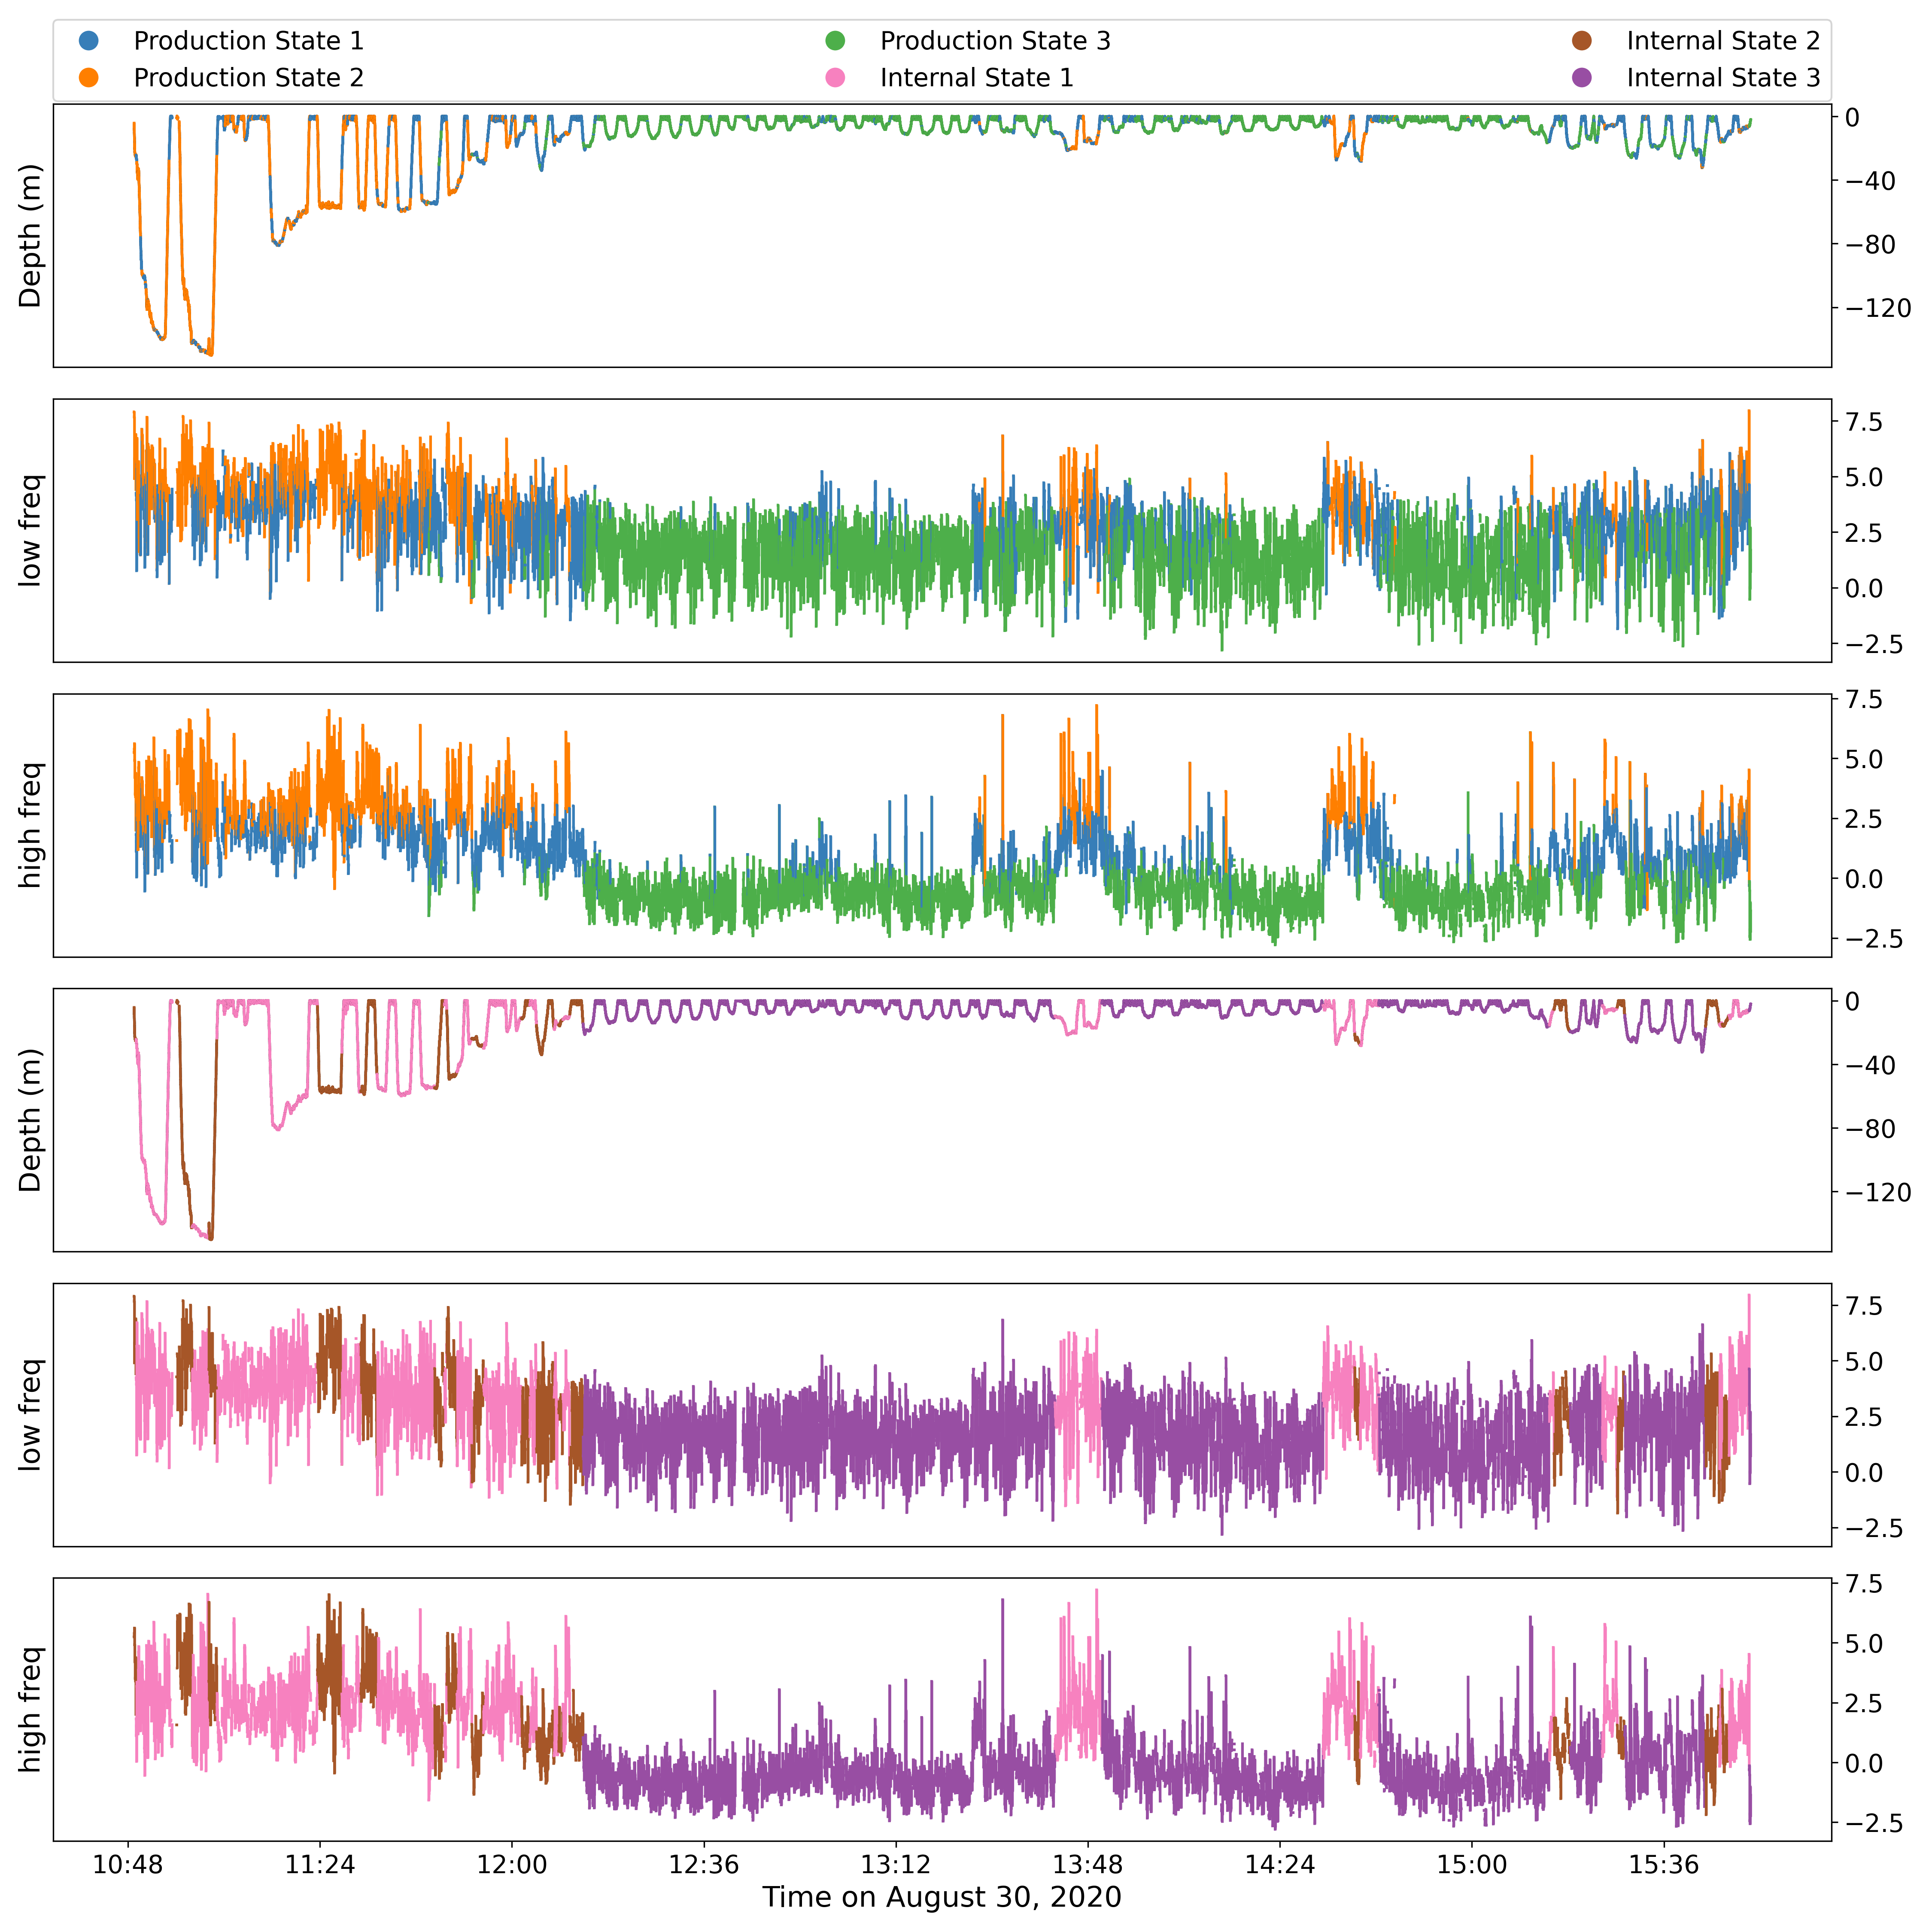
\includegraphics[width=6.5in]{plt/decoded_dives_kw_I145_K_3_3_nWhales_8.png}
    \caption{Dive profile and ``wiggliness" associated with a selected Killer Whale off the coast of British Columbia, Canada. Data is colour-coded according to the most likely hidden fine-scale state (top three panels) or coarse-scale state (bottom three panels) of each two-second window.}
    \label{fig:data}
\end{figure}
%
Fine-scale states 3, 1, and 2 appear to correspond to increasing activity, respectively. Coarse-scale states 1 and 2 appear to correspond to varying level of activity when the killer whale is hunting or socializing, while internal state 3 appears to correspond to resting behaviour.

We used a procedure similar to the simulation study to initialize the HMM parameters of the case study. Let $\bar y$ and $\bfQ$ denotes the sample mean and sample covariance of $\{y_t\}_{t=1}^T$, respectively. In all optimization procedures we initialized $\theta_0$ as
%
\begin{equation}
    \mu^{(i)}_0 \sim \calN(\bar y, \text{diag}(\bfQ)), \quad \Sigma^{(i)}_0 = \text{diag}(\bfQ), \qquad i \in \{1,\ldots,N^{(f)}\},
\end{equation}
%
Note that we only define emission distributions for $i = 1,\ldots,N^{(f)}$ because we assume that each coarse-scale state has the same fine-scale emission distributions.
Throughout the optimization procedure, we also assume that $\Sigma^{(i)}$ is diagonal for all $i \in \{1,\ldots,N^{(f)}\}$.
%
Let $\eta_k^{(c)}$ denote the parameters associated with the coarse-scale probability transition matrix at iteration $k$ of a given optimization algorithm. We initialized $\eta_0^{(c)}$ as
%
\begin{align}
    \eta^{(c,i)}_{0} &\sim \calN(0,1), & i & = 2,\ldots,N^{(c)} \\
    %
    \eta^{(c,i,j)}_{0} &\sim \calN(-2,2^2), & i,j & = 1,\ldots,N^{(c)}, \qquad i \neq j.
\end{align}
%
Further, let $\eta_k^{(f)}$ denote the parameters associated with the fine-scale transition probability matrices and fine-scale initial distributions at iteration $k$ of a given optimization algorithm. We initialized all elements of $\eta^{(f)}_{0}$ 
as follows:
%
\begin{align}
    \eta^{(f,i,i')}_{0} &\sim \calN(0,1), & i & = 1,\ldots,N^{(c)}, & i' & = 2,\ldots,N^{(f)} \\
    %
    \eta^{(f,i,i',j')}_{0} &\sim \calN(-2,2^2), & i & = 1,\ldots,N^{(c)}, & i',j' & = 1,\ldots,N^{(f)}, \qquad i' \neq j'
\end{align}
%
%If the 2-norm of the average estimated gradient $||\frac{1}{T}\sum_{t=1}^T \widehat \nabla F^{(k,m)}_t + \widehat \nabla G^{(k,m)}_t||$ ever fell below a tolerance of $10^{-8}$, we terminated the M-step of algorithm and moved on to the E-step. Likewise, if the relative change of the log-likelihood after one full E- and M- step of the EM algorithm ever fell below a tolerance of $10^{-10}$, we terminated the algorithm altogether. We found the ground truth MLEs by running the traditional EM algorithm until the relative change in the log-likelihood was on the order of machine precision $10^{-15}$.
%
Similarly to the simulation study, we estimated the parameters of the hierarchical HMM using our six inference algorithms and three baseline algorithms.
%
All algorithms were run using 50 random initializations for a total of 12 hours each on Compute Canada Cedar nodes with 16GB of RAM.

Figure (\ref{fig:ll_trace_case}) displays the log-likelihood (divided by $T$) of the maximum log-likelihood minus the log-likelihood (divided by $T$) at each epoch after 12 hours or 100 epochs (whichever came first). For each optimization algorithm, we present the random initialization that resulted in the highest likelihood after 12 hours of computation. The dots correspond to the epoch and likelihood at convergence for each algorithm.  Convergence is defined as the point at which the gradient norm of the log-likelihood (divided by $T$) was less than $10^{-2}$. We selected a tolerance of $10^{-2}$ because it was the lowest tolerance that all algorithms regularly converged to within 12 hours. 
%
\begin{figure}
    \centering
    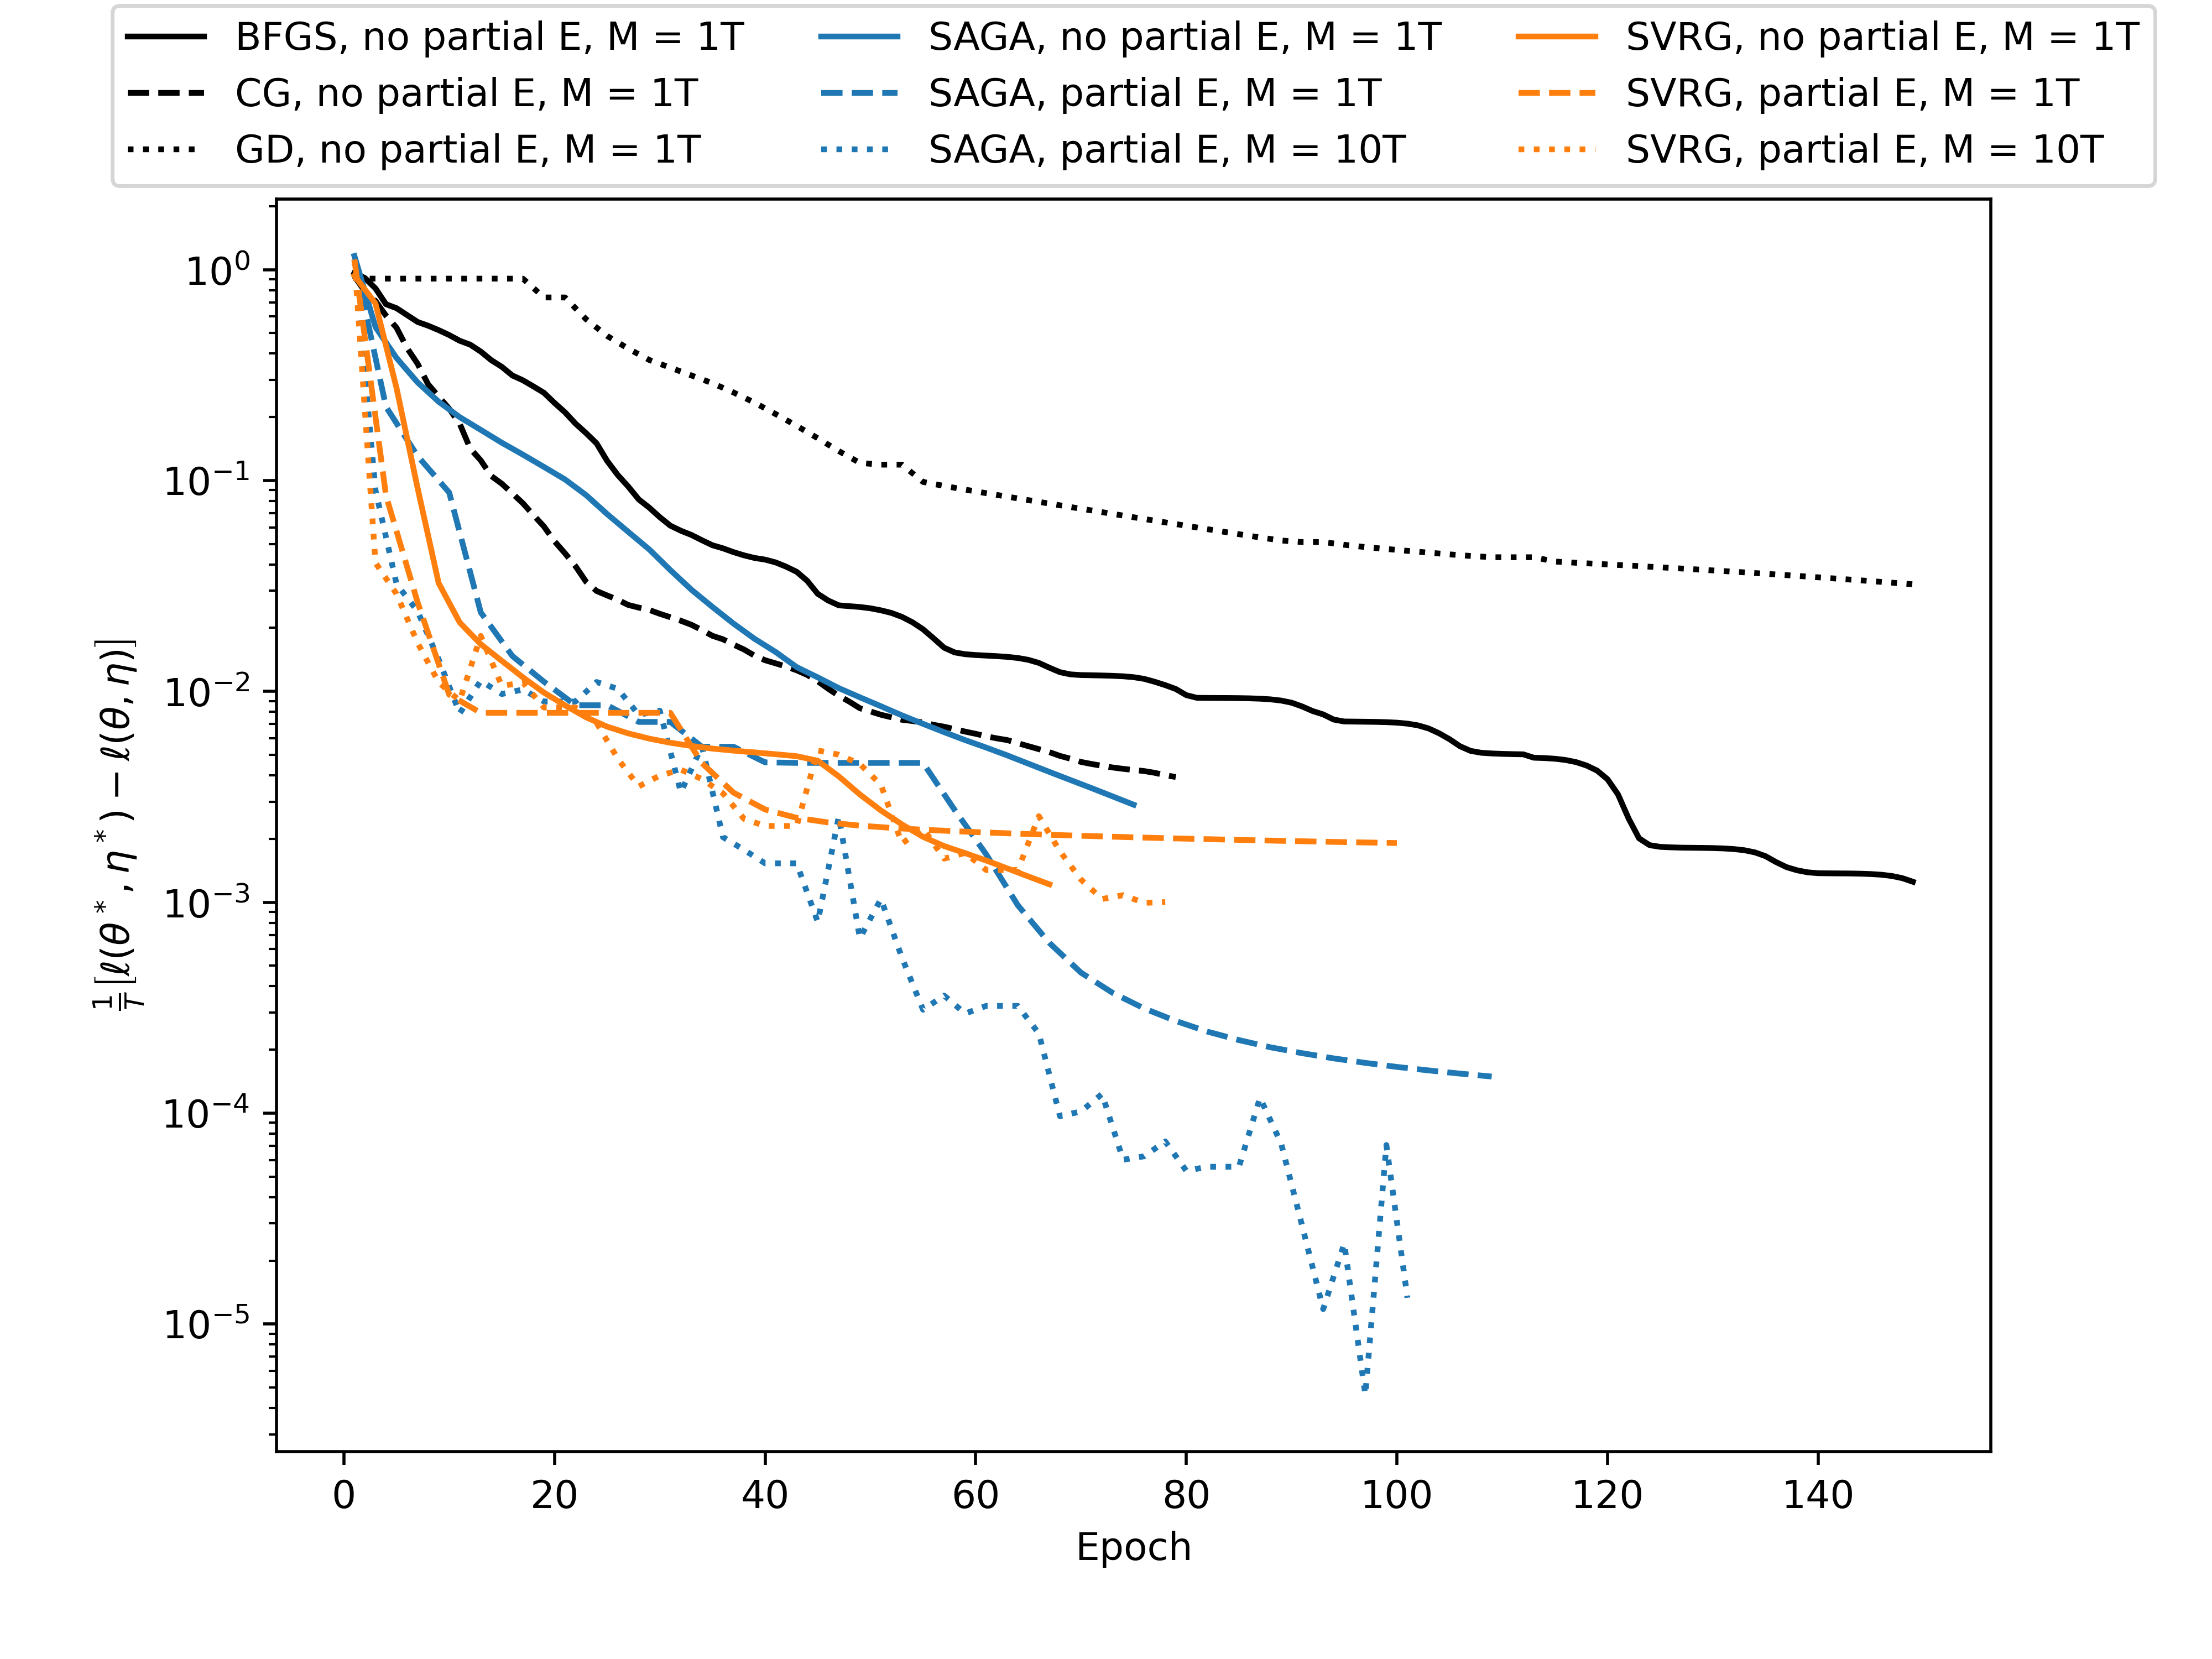
\includegraphics[width=6in]{../plt/log-like_v_epoch_K-3-3.png}
    \caption{Optimally gap between the log-likelihood and optimal log-likelihood for the estimated parameters of the HMM from the Killer Whale case study. One epoch represents either one full E-step, $T$ iterations with the M-step, or one gradient step for full-gradient algorithms. The y-axis is on a log-scale.}
    \label{fig:ll_trace_case}
\end{figure}

Figure (\ref{fig:boxplots_case}) shows box plots of both the number of epochs until convergence as well as the optimality gap (log likelihood divided by $T$) at convergence for each algorithm.
%
\begin{figure}
    \centering
    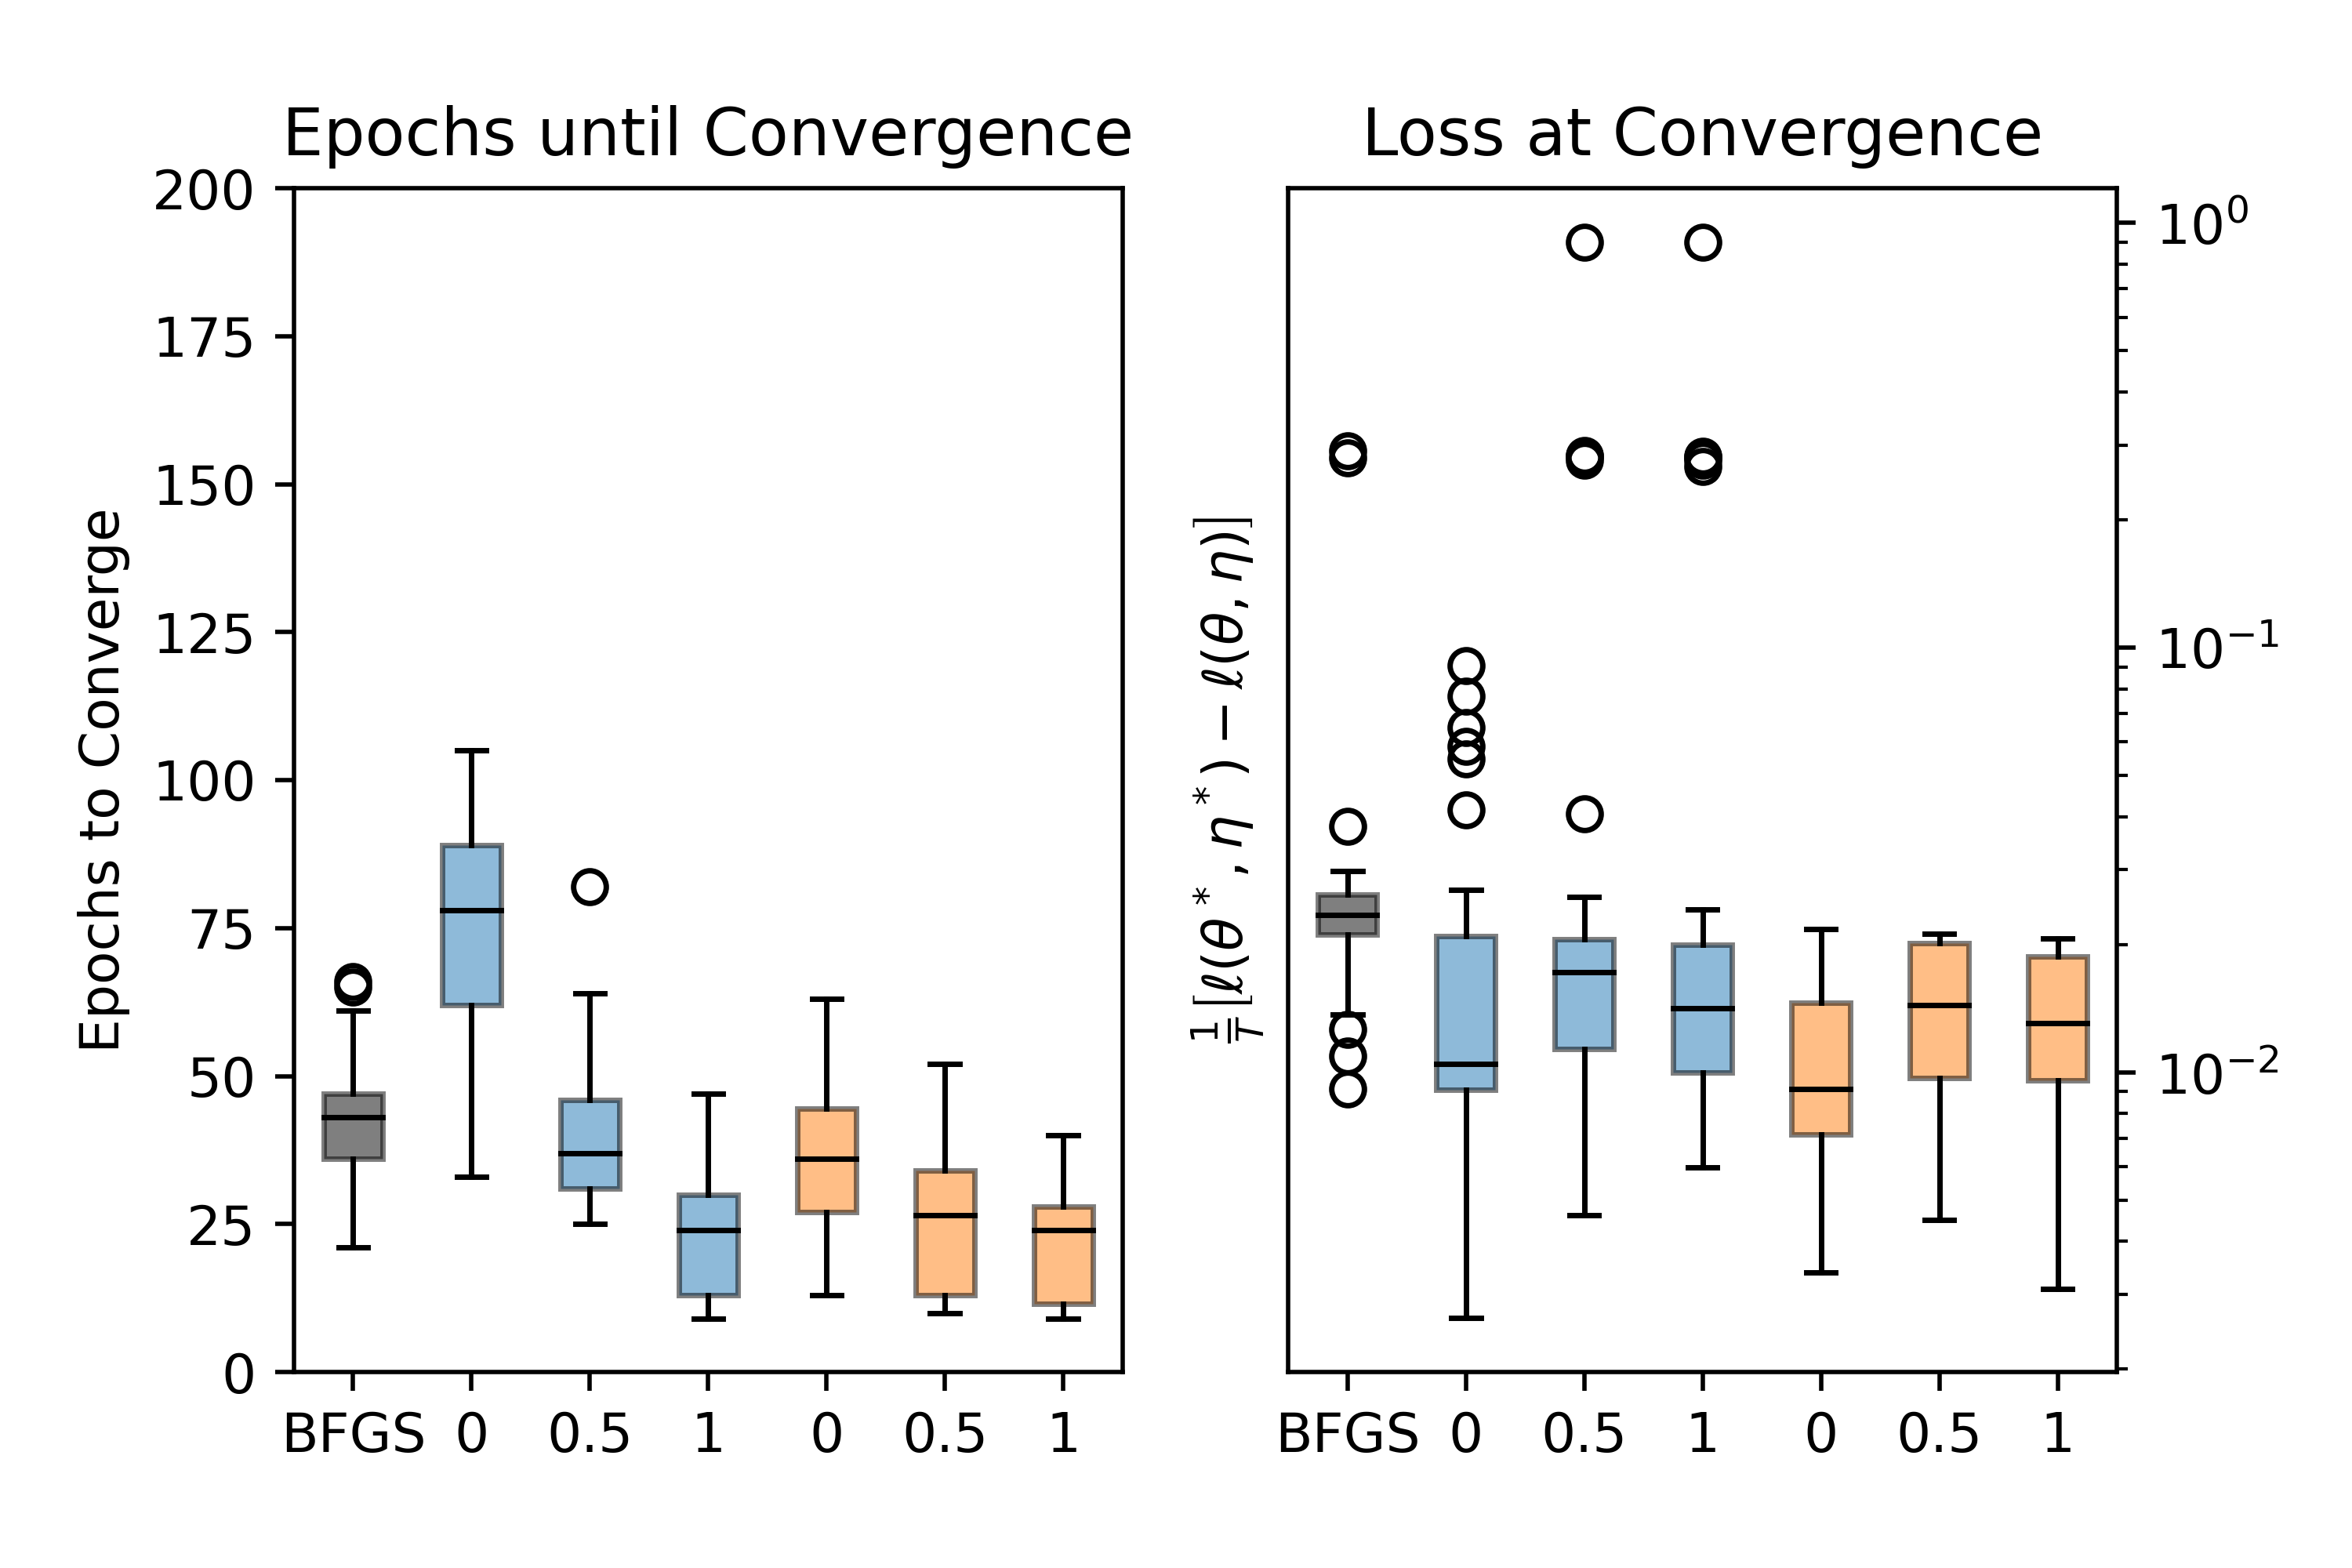
\includegraphics[width=6.5in]{../plt/boxplots_case_study.png}
    \caption{Box plots showing epochs to converge (left) and the optimality gap at convergence (right) for each optimization algorithm. NPE corresponds to algorithm (\ref{alg:EM-SO}), PE1 corresponds to algorithm (\ref{alg:P-EM-SO}) with $M=T$, and PE2 corresponds to algorithm (\ref{alg:P-EM-SO}) with $M=10T$. Blue corresponds to SAGA and orange corresponds to SVRG.}
    \label{fig:boxplots_case}
\end{figure}
%
All of the algorithms presented in this paper converge with higher likelihood than BFGS (on average), and all algorithms except for algorithm (\ref{alg:P-EM-SO}) with SAGA tend to converge in fewer epochs than BFGS.

Figure (\ref{fig:scatter_case}) displays scatter plots of the number of epochs to converge and the loss at convergence of each algorithm vs. BFGS for the same data set and parameter initializations.
%
\begin{figure}
    \centering
    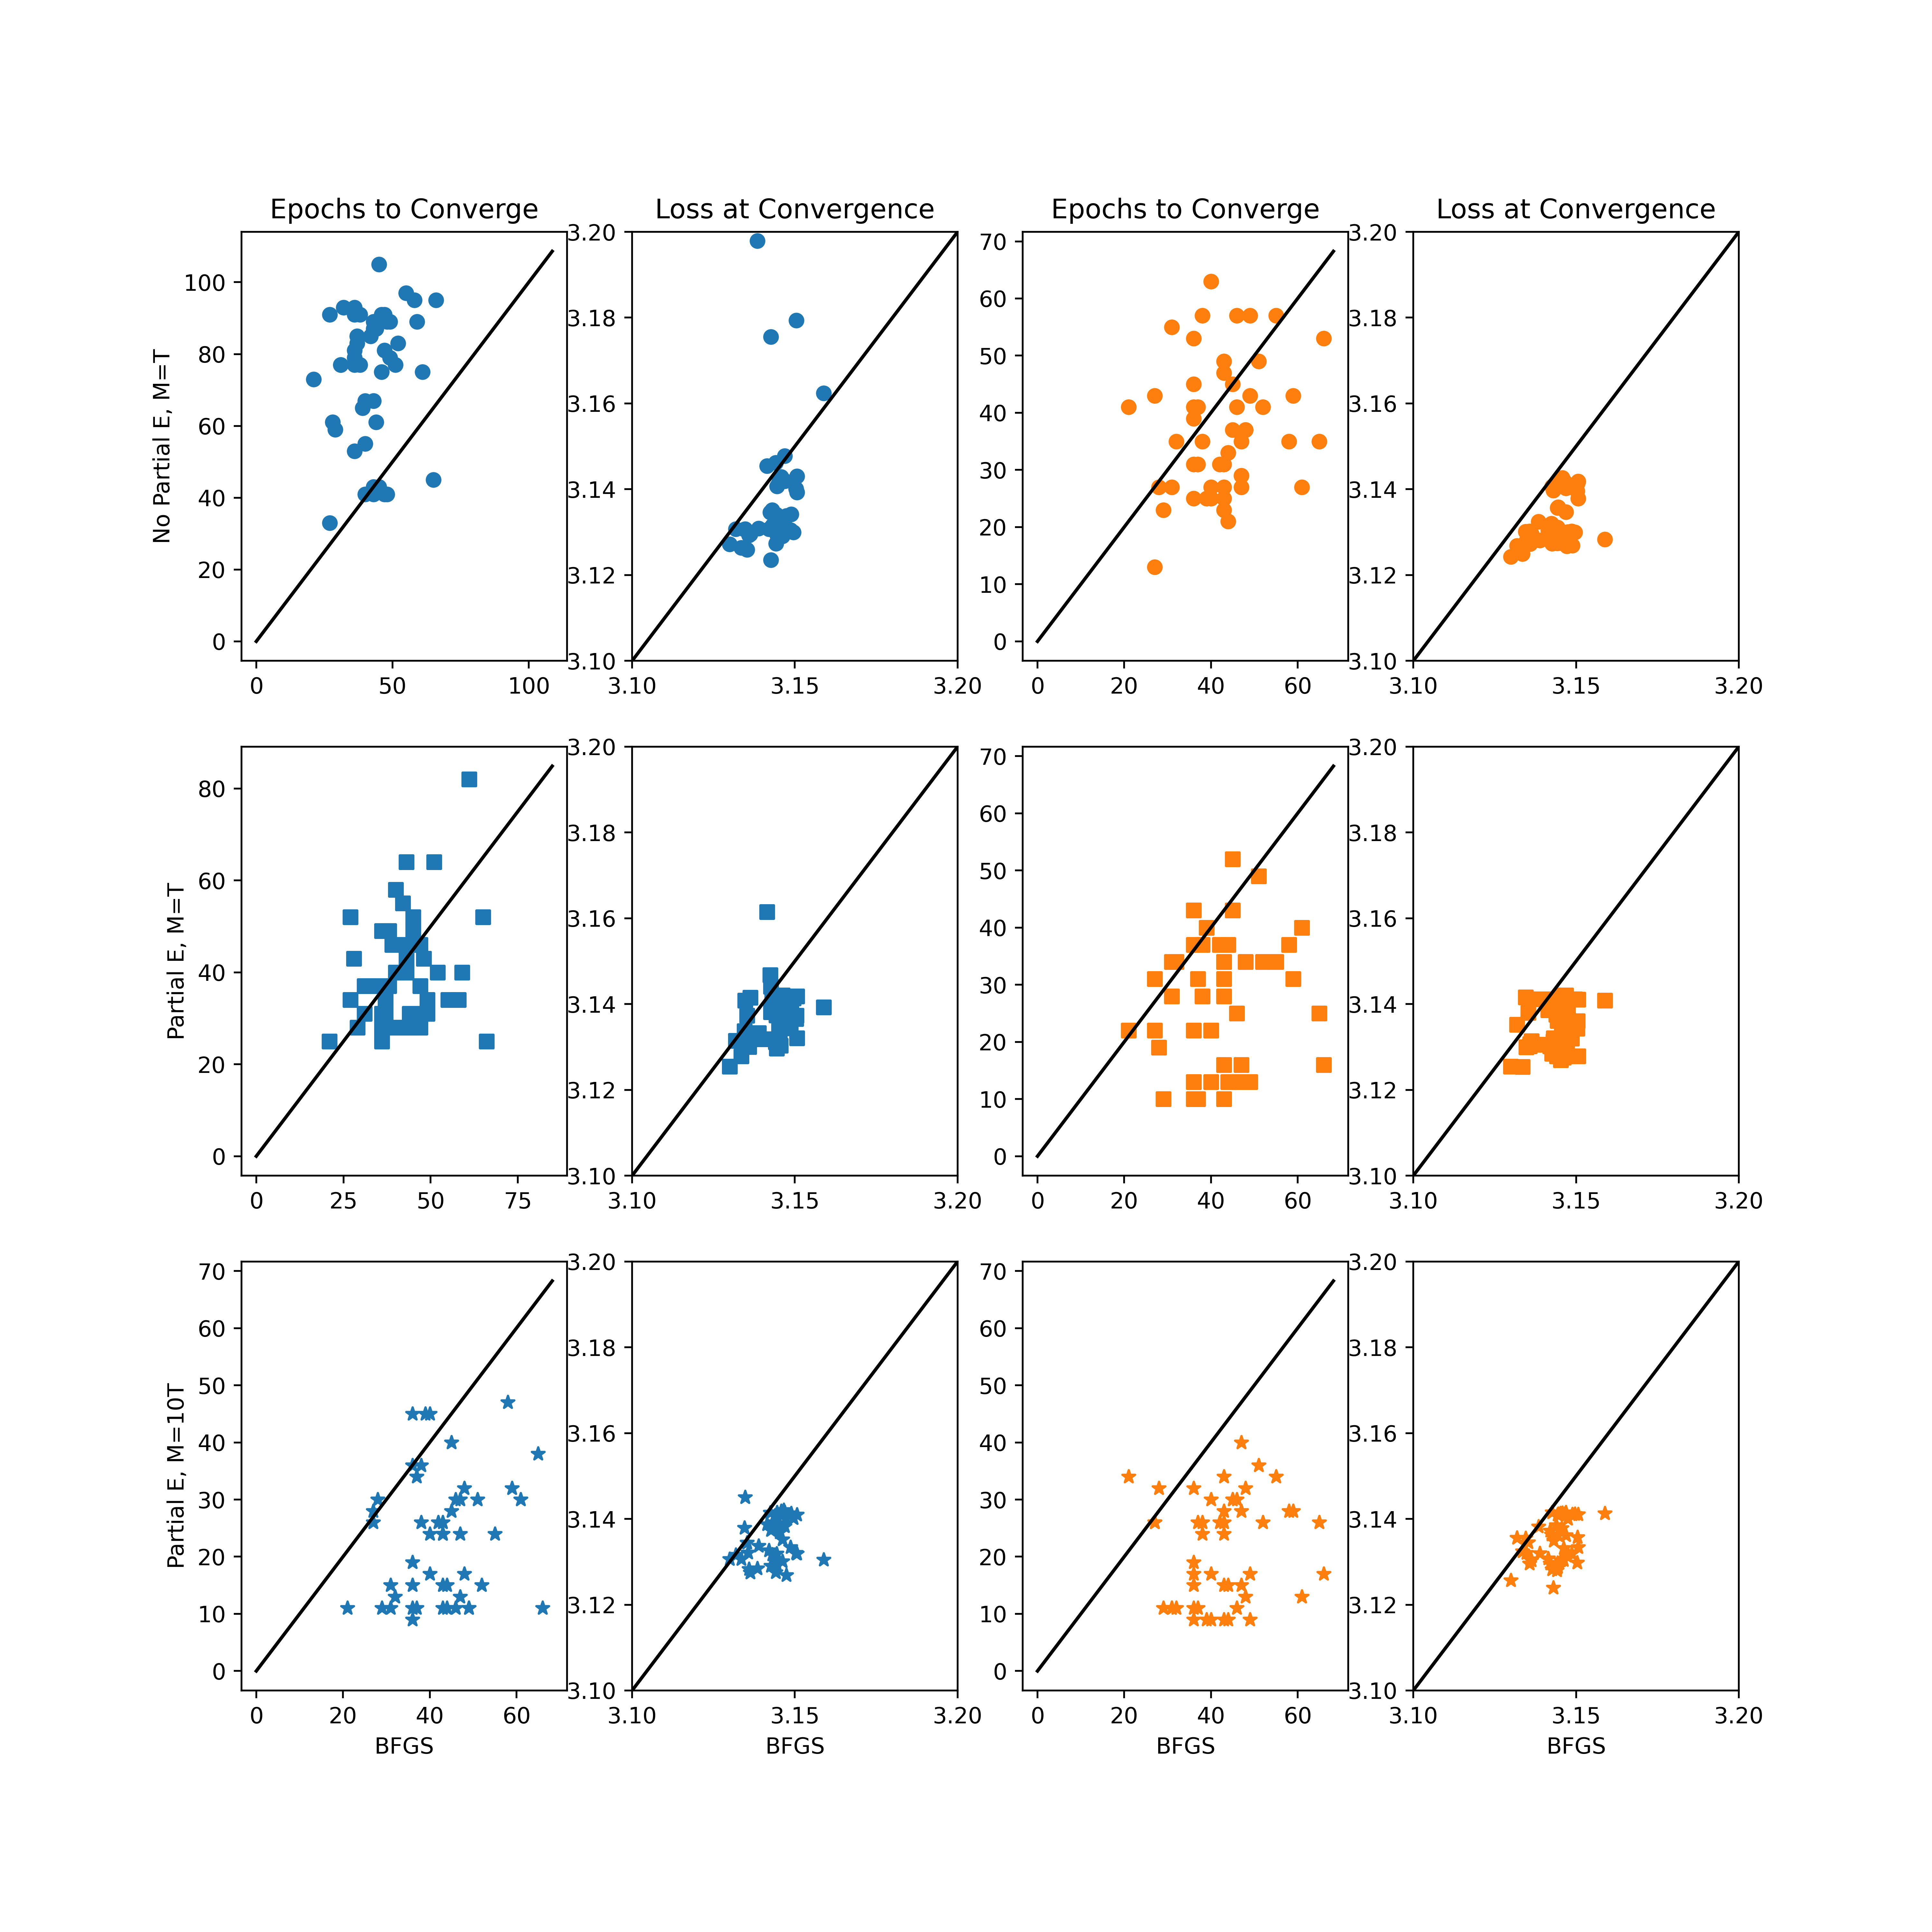
\includegraphics[width=6.5in]{../plt/paired_scatter_case_study.png}
    \caption{Number of epochs to converge (columns 1 and 3) and the loss at convergence (columns 2 and 4) of each algorithm vs. BFGS for identical data sets and parameter initializations. Lower is better for both criteria, so data points below the line $y=x$ suggest that the stochastic optimization algorithms perform better.}
    \label{fig:scatter_case}
\end{figure}
%
Like the simulation study, SVRG appears to converge faster than SAGA for all algorithms. %This may be a function of our step size ($1/3 \hat L$), but that step size was selected based upon suggestions from the SAGA paper \citep{Defazio:2014}. In addition, 
All of our stochastic optimization algorithms converge faster than BFGS, except for algorithm (\ref{alg:EM-SO}) with SAGA. However, all stochastic optimization algorithms tend to converge to areas of lower loss than BFGS. 

%SAGA without a partial E-step performs similarly to the EM algorithm in a per-epoch basis because SAGA is successfully converging for the M-step when $M = T$. However, it does not perform as well as the EM algorithm on a per-time basis because the M-step is significantly slower when using SAGA vs the closed-form solution. This behaviour is expected, and SAGA has a significant advantage over the EM algorithm in that it only requires gradients rather than sufficient statistics.

%mplementing a partial E-step shows that SAGA can outperform the EM algorithm when the parameter estimates are far from the optimal solutions and when the underlying HMM does not mix rapidly. This is likely because the weights of the $F$ and $G$ are very inaccurate at first, and updating them early in the optimization procedure yields a significant speed-up. In addition, if the Markov chain is rapidly mixing, then updates to $\gamma_{t_m}$ and $\xi_{t_m}$ at a single data point are more accurate. Future work may involve performing the partial-E step for many weights at once sequentially, depending upon the mixing time of the current estimate of $\eta_k$.